\section{Results}
\label{sec:results}

In this section we present the outcome of our implementation.



%% --------------------------------------------

\subsection{Markov Chains}
\label{subsec:markovchains}
We ran each of our Markov chains over 5000 iterations.

%% --------------------------------------------

\subsubsection{Proposals}
\label{subsec:proposals}

\begin{table}
  \centering
  \caption{Proposals used by our Markov Chains}
  \label{tbl:proposals}
  \begin{tabular}{lr}
    \toprule
      \textbf{Update Proposal} &
      Standard Deviation \\
    \midrule
      Tiny Shape & 0.02 \\
      Small Shape & 0.05 \\
      Medium Shape & 0.1 \\
      Large Shape & 0.3 \\
      Rotation & 0.01 \\
      Translation & 1.0 \\
    \bottomrule
  \end{tabular}
\end{table}

The proposals we used in our Markov Chains can be seen in \autoref{tbl:proposals}. For the different combinations of said proposals  please see \autoref{tbl:markovchains}.

\begin{table}
  \centering
  \caption{Weight combinations of proposals for the Markov Chains}
  \label{tbl:markovchains}
  \begin{tabular}{lrrr}
    \toprule
      \textbf{Update Proposal} &
      Chain 1 &
      Chain 2 &
      Chain 3 \\
    \midrule
      Tiny Shape & 0.0 & 0.0 & 0.2 \\
      Small Shape & 0.1 & 0.3 & 0.5 \\
      Medium Shape & 0.2 & 0.4 & 0.2 \\
      Large Shape & 0.1 & 0.1 & 0.0 \\
      Rotation & 0.3 & 0.1 & 0.05 \\
      Translation & 0.3 & 0.1 & 0.05 \\
    \bottomrule
  \end{tabular}
\end{table}
%% --------------------------------------------

\subsection{Test Fit}
\label{subsec:testfit}
As we were given the ground truth model for the test CT images, we were able to calculate the average and hausdorff distance from our calculated model to the true model, as seen in \autoref{tbl:testfit}. 

\begin{table}
  \centering
  \caption{Test fit distance to ground truth}
  \label{tbl:testfit}
  \begin{tabular}{lrr}
    \toprule
      \textbf{Bone Image} &
      Average Distance &
       Hausdorff Distance \\
    \midrule
      Bone 4 & 0.57 & 4.98 \\
      Bone 14 & 0.41 & 2.23 \\
      Bone 23 & 0.59 & 3.16 \\
      Bone 25 & 0.71 & 5.24 \\
      Bone 30 & 0.51 & 2.94 \\
    \midrule
      Average & 0.56 & 3.71 \\
      Standard Deviation & 0.11 & 1.33 \\
    \bottomrule
  \end{tabular}
\end{table}

\begin{figure}
	\centering
  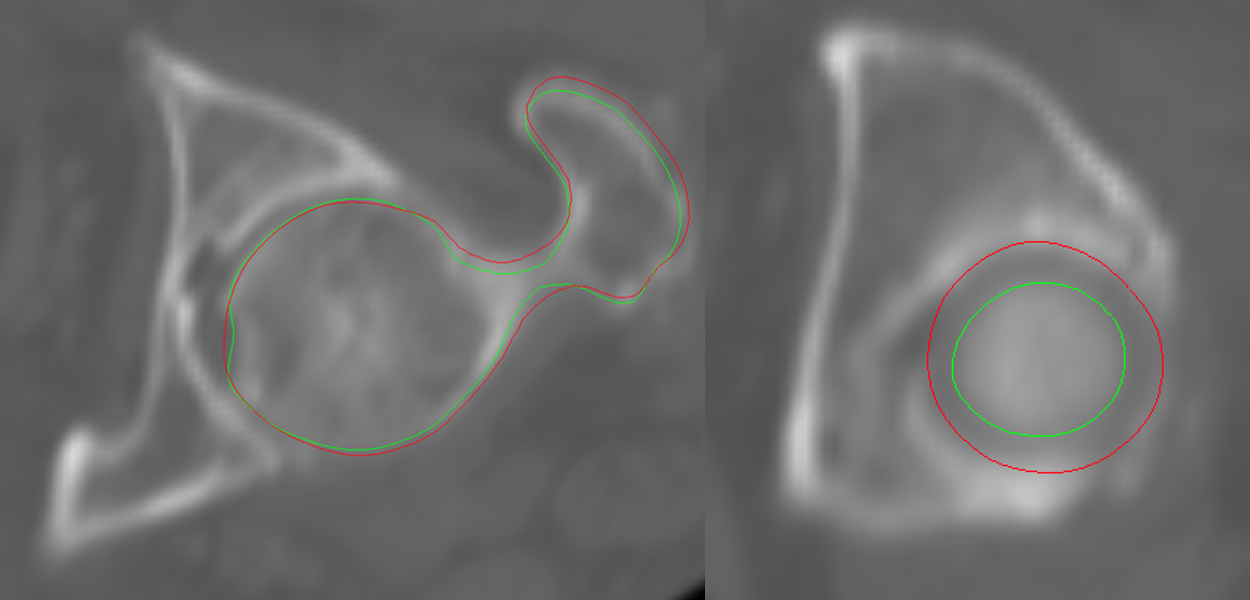
\includegraphics[width=\columnwidth]{./Figures/local_minimum_comparison}
  \caption{
    Left: Example of our model escaping a local minimum. Right: Example of our model getting stuck in a local minimum}
  \label{fig:testfit}
\end{figure}

\subsection{Target Fit}
Of course we can not provide average distances for the target fits, however an example image of one of our fits can be seen in \autoref{fig:targetfit}.

\begin{figure}
	\centering
  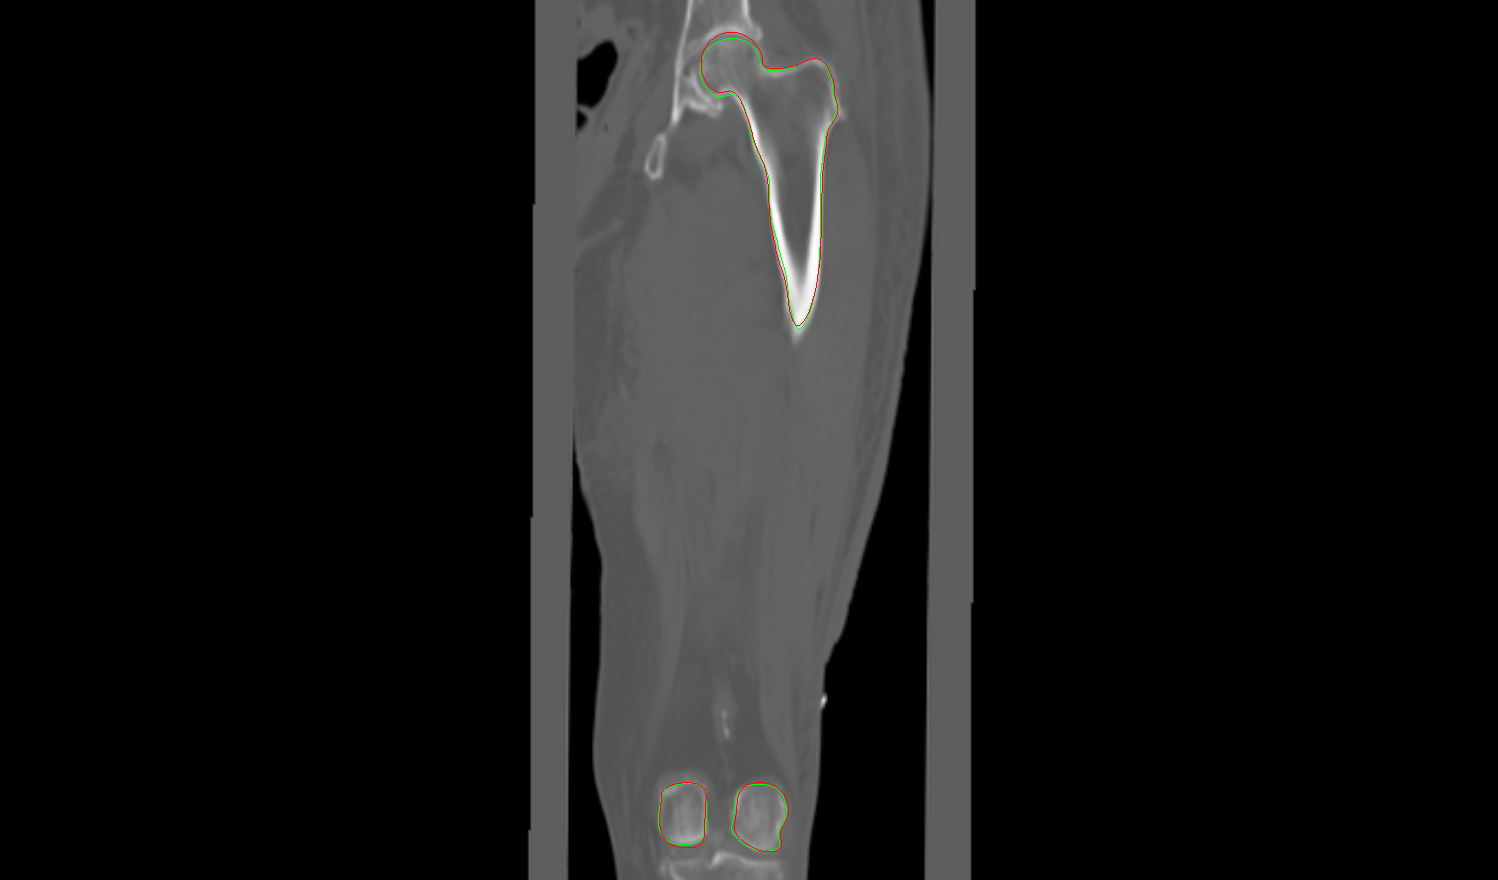
\includegraphics[width=\columnwidth]{./Figures/local_minimum_y-axis}
  \caption{
    Example of a fit of our model to the target CT image. }
  \label{fig:targetfit}
\end{figure}
\todoRevise{Figure with target fit}